\documentclass[11pt]{article}
\PassOptionsToPackage{hyperfootnotes=false}{hyperref}
\usepackage[preprint]{acl}
\usepackage{times}
\usepackage{latexsym}
\usepackage[T1]{fontenc}
\usepackage[utf8]{inputenc}
\usepackage{microtype}
\usepackage{graphicx}
\usepackage{amsmath,amssymb}
\usepackage{booktabs,tabularx,array}

\title{Jev for Scientific Decisions:\\Evaluating Semantic Choices and Their Consequences}

% Author order follows the supplied template. Affiliations await author input.
% Change preprint to review above for an anonymous submission PDF.
\author{
 \textbf{Boyuan Deng\textsuperscript{1}}\thanks{Corresponding author},
 \textbf{Shuyi Fan\textsuperscript{2}},
 \textbf{Hongyang Zhang\textsuperscript{3}},
 \textbf{Xinhong Xie\textsuperscript{4}}\\
 \textsuperscript{1}Johns Hopkins University, \textsuperscript{2}Columbia University\\
 \textsuperscript{3}The Hong Kong Polytechnic University, \textsuperscript{4}The Pennsylvania State University
}

\begin{document}
\maketitle

\begin{abstract}
    Scientific workflows often require choosing among known relations before a deterministic calculation can proceed. Whether observations share a culture, treatment or reference standard can change the scientific meaning of the resulting count or comparison. We evaluate Jev as a semantic decision component using a harness that follows its documented guidance and assigns arithmetic to code. The study compares twelve model configurations on twenty source-grounded Choices across ten scientific cases, each repeated five times. We measure semantic selections, downstream outputs and final claim labels separately. Jev matched five other configurations at complete semantic correctness and achieved the lowest observed median latency among successful responses. Across three comparison models, seven wrong selections on one culture-history question changed downstream counts while preserving the correct final label. These results identify a useful role for Jev in prepared scientific decision tasks and show why evaluating that role requires checking the relations and quantities that a workflow will reuse.
\end{abstract}

\section{Introduction}
\label{sec:introduction}

Scientific workflows often turn on small decisions about what an observation represents. Ten measurements may describe independently grown cultures or repeated samples from a single culture. That distinction determines what a program should count and which claims the evidence supports. Similar decisions arise when identifying shared calibration standards, paired simulations or experimental assignments. Their answer spaces can be finite even when selecting the appropriate relation requires interpreting scientific language.

This interface between language and computation is a natural setting for Jev, a model designed to answer typed questions about supplied state \citep{typesafe2026introduction}. Its Choice interface selects from explicit candidates \citep{typesafe2026choice}. The documented division of labor assigns numerical operations to code and semantic judgments to the model \citep{typesafe2026jaggedness}. For scientific applications, the practical question is whether these judgments remain correct at useful request cost and latency, and whether their downstream consequences are captured by evaluation.

Scientific question answering and claim verification already provide relevant evaluation settings. PubMedQA pairs research questions with abstract context \citep{jin2019pubmedqa}, and Jevals uses a binary version to evaluate Jev \citep{jevals2026methodology}. SciFact evaluates scientific claims together with supporting evidence \citep{wadden2020fact}. More recently, \citet{ho2025table} showed that correct scientific claim labels can coexist with incorrect cell-level rationales. We examine executable relations: a selected relation controls a specified calculation, exposing whether a correct label accompanies a correct scientific output.

We contribute source-grounded scientific decision materials, a shared harness implementing the documented code--model division, and a comparison of Jev with eleven other configurations. Our analysis connects semantic correctness to derived outputs and final labels, and compares request latency and response cost. This provides concrete evidence for choosing a model at a bounded decision point within a scientific workflow.

\section{Scientific Decisions and Evaluation}
\label{sec:evaluation}

\subsection{Cases and the shared harness}
\label{sec:cases}

The model comparison uses twenty scientific Choices in ten cases, with two questions per case. The questions concern experimental units, shared histories, dependence and protocol applicability. Sources span manufacturing and materials, physical simulations, climate, metrology and biological experiments. These cases belong to a development collection of forty scientific Choices in twenty case groups, plus one engineering control. Passage-specific code rules resolve the other twenty scientific Choices without a model call. Appendix~\ref{app:cases} explains the question types, scientific cases and reference interpretations.

Each model receives the same prepared evidence passages, structured records, question instructions and candidate meanings. The packets contain source-grounded adaptations and transcriptions; reference answers and the constructed claims being assessed are kept outside model inputs.

Following Jev's guidance, the harness asks atomic questions, points each question to the supplied evidence and keeps counting, filtering, arithmetic and label composition in code. Jev uses its native Choice interface; the other models return candidate identifiers through a constrained JSON schema. Both questions are submitted together. This shared contract holds the evidence and downstream program fixed across models.

\begin{figure*}[t]
  \centering
  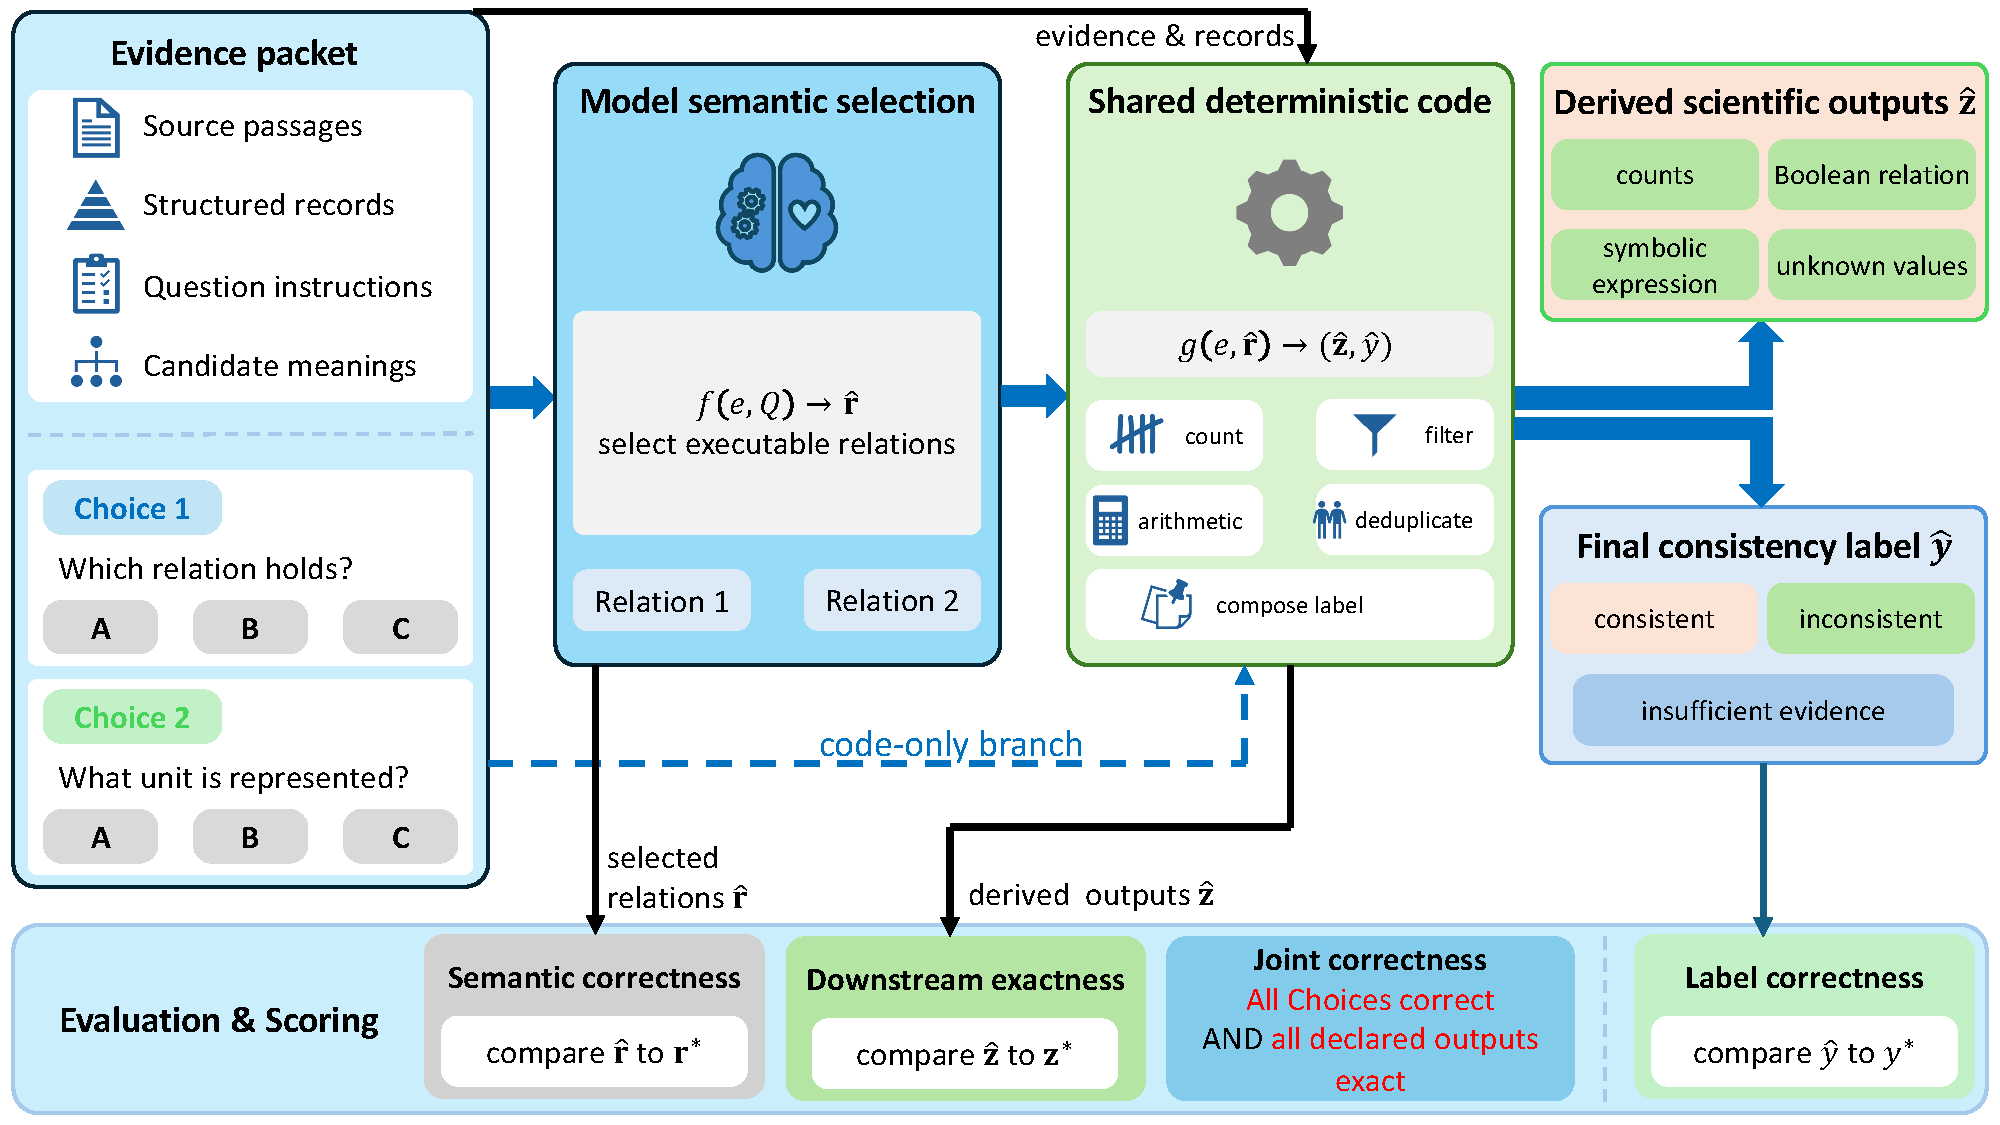
\includegraphics[width=0.95\textwidth]{jev4sci.pdf}
  \caption{Evaluation at a scientific decision point. The model selects relations from supplied evidence; shared code derives scientific outputs and composes a claim label. We score the selected relations, declared outputs and final label against separate references. The code-only branch bypasses the model.}
  \label{fig:workflow}
\end{figure*}

\subsection{Three levels of correctness}
\label{sec:metrics}

Let $e$ denote the supplied evidence and records, and $Q$ the questions with their candidate relations. The model $f$ selects a relation for each Choice, yielding $\hat{\mathbf r}$. The shared deterministic program $g$ applies the case's computation and claim-assessment rules to produce scientific outputs $\hat{\mathbf z}$ and a final label $\hat y$:
\begin{equation}
 \hat{\mathbf r}=f(e,Q),\qquad
 (\hat{\mathbf z},\hat y)=g(e,\hat{\mathbf r}).
 \label{eq:workflow}
\end{equation}
Figure~\ref{fig:workflow} shows this division. The reference relations, outputs and label are $\mathbf r^*$, $\mathbf z^*$ and $y^*$.

\textbf{Semantic correctness} requires the selected candidate for Choice $k$ to match its reference exactly: $\hat r_k=r_k^*$. \textbf{Downstream exactness} requires agreement on every declared scientific output for a case, including counts, Boolean relations, symbolic expressions and unknown values. These fields exclude claim assessments and labels. \textbf{Label correctness} requires $\hat y=y^*$ for the canonical final label. We also report \textbf{joint correctness}, requiring all semantic selections and downstream outputs to agree. Appendix~\ref{app:metrics} specifies the output fields and scoring procedure.

These checks answer different questions. The program in Equation~\ref{eq:workflow} can map distinct relations to the same quantities or final label. Conversely, it can execute a wrong relation exactly and produce a wrong scientific result. All ten model-routed reference cases have the final label \texttt{inconsistent}; an always-\texttt{inconsistent} baseline therefore solves the label task. Semantic and joint correctness provide the substantive quality comparison.

\subsection{Experimental comparison}
\label{sec:setup}

We compared twelve configurations on all ten cases, each repeated five times. Each configuration therefore had fifty planned requests and one hundred semantic answers. Configurations were evaluated in three groups, with serial requests, shuffled case order and rotating model order within each group. Repetitions measure variation on the same inputs; the scientific sample remains ten cases containing twenty Choices.

The primary scores use the planned denominators, with no replacement of missing responses. An absent response earns no correctness credit and is distinguished from a wrong selection. We also report correctness conditional on receiving an answer (Appendix~\ref{app:observed}). Each request was evaluated once, without retries or provider substitution. Model versions and inference settings are specified in the accompanying code and results.

Latency measures elapsed client request time; we report its median and nearest-rank 95th percentile among successful responses. Cost is the known mean charge per successful response, using provider-reported charges or estimates from token usage and the applicable prices. These measurements describe the evaluated configurations under their respective service conditions.

\begin{table*}[t]
\centering
\small
\begin{tabular*}{\textwidth}{@{\extracolsep{\fill}}lrrrrrrr@{}}
\toprule
 & \multicolumn{4}{c}{Correctness and availability} & \multicolumn{3}{c}{Successful-request resources} \\
\cmidrule(lr){2-5}\cmidrule(l){6-8}
Model & Returned & Semantic & Downstream & Label & Median & p95 & Cost \\
 & /50 & /100 & $=$ Joint /50 & /50 & (s) & (s) & (\$/1,000) \\
\midrule
\csname @@input\endcsname analysis/main_table_rows.tex
\bottomrule
\end{tabular*}
\caption{Comparison on twenty Choices in ten cases, repeated five times per configuration. Returned counts complete responses; correctness uses planned denominators and gives no credit for missing responses. Downstream and joint counts coincide in these results. Cost is the known mean successful-response cost per 1,000 requests; $r$ denotes reported charges and $e$ usage-based estimates. Preparation costs and unmeasured charges are excluded.}
\label{tab:main}
\end{table*}

\section{Results}
\label{sec:results}

\subsection{Decision quality}

Jev answered all one hundred planned semantic questions correctly and obtained all fifty downstream results (Table~\ref{tab:main}). GPT-5.6 Sol \citep{openai2026gpt56}, GPT-6 Astra \citep{openai2026gpt6astra}, Claude Sonnet 5 \citep{anthropic2026sonnet5}, Claude Opus 5 \citep{anthropic2026opus5} and Kimi K3 \citep{moonshot2026kimik3} achieved the same scores. Luna made one wrong selection, Qwen Flash \citep{qwen2026flash} one and Qwen Max \citep{alibaba2026qwen38max} five. All seven concerned the same culture-history question. Downstream and joint correctness coincided for the observed responses.

Response coverage and answer quality differed for several configurations. Terra and DeepSeek configurations \citep{deepseek2026v41flash,deepseek2026v4pro0813} answered every received question correctly, but missing responses reduced their planned-denominator scores. Conditional scores in Appendix~\ref{app:observed} distinguish these coverage differences from semantic errors.

\subsection{Correct labels can conceal wrong quantities}
\label{sec:errors}

The culture-history case uses the experiments of \citet{luria1943mutations}. Ten samples in column 11a come from one culture; ten in column 11 come from separately grown cultures. Their growth-history counts are $(1,10)$. The question asks whether samples within each series share a culture history.

The seven wrong selections produced $(10,1)$ four times, $(1,1)$ twice and $(10,10)$ once. In every response, the second Choice correctly identified colonies as clonal descendants. This rejected the claim that each colony represented an independent mutation origin. The final label remained \texttt{inconsistent} despite the wrong growth-history counts.

Across the 588 received results, all final labels were correct, while 581 downstream outputs were exact. This difference represents seven responses on one scientific question. It exposes a concrete failure that a label-only comparison would miss: the workflow can return the expected verdict while passing an incorrect quantity to subsequent analysis.

\subsection{Request latency and cost}

Jev had the lowest observed successful-request median latency, 0.335\,s, with a p95 of 0.442\,s. Its known mean cost was approximately \$0.000060 per successful response. Among configurations with complete semantic correctness and response coverage, the next lowest median was Sol's 1.385\,s; Sol also had the next lowest cost, \$0.003047 per successful response. Thus Jev combined the same observed correctness with lower request resource use in this collection.

\section{Implications for Scientific Workflows}
\label{sec:discussion}

The comparison supports Jev as a candidate component where evidence has been prepared, candidate relations are explicit and downstream operations are specified. Its observed request economy is useful for this recurring interface between scientific text and executable rules. Preserving the semantic selections also makes it possible to inspect which relation caused a downstream discrepancy.

The culture case extends the rationale--label distinction studied by \citet{ho2025table} to quantities that a scientific workflow could reuse. A final verdict compresses multiple clause judgments; one correctly rejected clause can conceal an error elsewhere. Evaluations of fixed-choice scientific components should therefore retain both relation-level references and the declared downstream outputs. Joint scoring checks whether the component supplies the correct relations as well as the expected result.

\section{Conclusion}

We evaluated Jev on prepared scientific decisions using shared deterministic computation and a twelve-configuration comparison. Jev combined complete observed semantic correctness with the lowest recorded successful-request median latency and known mean response cost. Separating semantic selections, downstream outputs and final labels revealed errors hidden by the final verdict, yielding a practical evaluation contract for scientific decision components.

\section*{Limitations}

The comparison uses a development collection of twenty model-routed Choices in ten cases. The same curated English packets recur across repetitions, and six configurations achieve complete correctness. All observed semantic errors concern one Choice. This design characterizes the supplied decisions; evaluating transfer requires new, source-separated cases and broader relation coverage.

Every model-routed reference label is \texttt{inconsistent}, and none of its reference Choices is \texttt{not\_stated}, \texttt{other} or \texttt{conflicting}. The collection therefore measures relation selection and its consequences within these cases. Balanced claim decisions and uncertain-evidence cases are needed to assess label discrimination and abstention. Declared downstream outputs summarize selected scientific consequences; semantic scoring remains necessary when different relations yield identical outputs.

The evaluation begins with supplied evidence passages and structured records. The harness comparison uses one implemented configuration per model; its component effects would require a separate ablation study.

Latency and cost depend on services, execution windows, reasoning settings and cache states. The resource comparison covers successful model requests. Charges for missing responses, data preparation costs and local computation costs are unmeasured, leaving total workflow expenditure undetermined.

\bibliography{references_verified,case_sources}

\appendix
% Requires booktabs. Include after \appendix in the main manuscript.
\section{Scientific questions and case construction}
\label{app:cases}

The collection contains 20 groups, 40 scientific Choices, and 25 claim outcomes.
A group shares evidence across related questions and can support more than one claim.
Ten groups, comprising 20 scientific Choices, follow deterministic rules developed on the prepared passages.
The other ten groups each contain two model-routed Choices.
Tables~\ref{tab:code-cases} and~\ref{tab:model-cases} list the complete collection and the resulting computations.
One additional candidate-omission check accompanies D01 and is excluded from scientific scores.
The 21 source records belong to 18 documented source families; related documents from the same experiment remain in one family.

\subsection{Relations that determine scientific quantities}

Several cases ask which scientific unit a recorded observation represents.
Specimens can share a build or mixing operation, scans can repeat one wear event, and minute-level measurements can share one controller allocation.
Likewise, a pooled library combines contributors, and a cosmological pair contributes one average despite requiring two simulation executions.
These distinctions determine which observations can be counted separately for the stated calculation.

Other cases ask how a unit's history or relationship to another unit affects interpretation.
Examples include catalyst reuse, mixed powder histories, shared culture growth, outcome-adaptive stress selection, and complementary treatment allocation.
Shared calibration uncertainty and bundled climate-model changes affect the interpretation of comparisons even when the number of reported results is unchanged.

A further recurring question is what the evidence identifies at the selected scope.
Exposure windows distinguish administration from developmental exposure, while allele diversity in mosaic founders leaves validated germline transmission unresolved.
Incomplete provenance can establish a mixture while leaving its exact parent-lot count unknown.
Each case links a relation judgment to the quantities supported by the evidence.

\begin{table*}[t]
\centering
\footnotesize
\setlength{\tabcolsep}{4pt}
\begin{tabular}{@{}p{0.06\textwidth}p{0.13\textwidth}p{0.28\textwidth}p{0.27\textwidth}p{0.18\textwidth}@{}}
\toprule
Group & Domain & Relation or unit & Derived scientific quantity & Source \\
\midrule
D01 & Concrete & Mixing operation and shared prism membership & One mixing operation, three prisms, six half-prisms & \citep{rezazadeh2026dataset} \\
D02 & Additive manufacturing & Complete build versus specimens within it & One build for three selected specimens & \citep{SHANBHAG2021107613} \\
D03 & Concrete curing & Bath-level control, run boundaries, specimen assignments & Curing-run count remains unknown & \citep{rezazadeh2026dataset} \\
C01 & Electroplating & Whole-plot unit for temperature/concentration; strip for current & One whole plot per setting; two strips per current level & \citep{nistUndatedNested} \\
H01 & Additive manufacturing & Column-level laser settings versus specimen-level heat treatment & Five selected columns; one heat-treated specimen & \citep{weaver2021demonstration} \\
C02 & Measurement systems & Wear-scar generation versus repeated scans & Two wear events identified by cutter--scar keys & \citep{wigginsUndatedMeasurement} \\
E001 & Semiconductor processing & Crossed implant/anneal memberships; wafer interaction unit & 64 setting combinations, one wafer each & \citep{nistUndatedNested} \\
E002 & Wind energy & Hourly controller switch and transition exclusion & Minute records do not add allocations; campaign count unknown & \citep{simley2021results} \\
E003 & Catalysis & Recovered catalyst carried between reaction cycles & Eight cycles in one documented reuse series & \citep{rafi2020copper} \\
E008 & Chemical process design & Equality of all eight coded factor settings & 20 runs, 18 distinct settings, two pure-error degrees of freedom & \citep{stallrich2026powerful,nistUndatedFoldover} \\
\bottomrule
\end{tabular}
\caption{Scientific relations and derived quantities for the ten groups resolved by deterministic rules developed on the prepared passages.}
\label{tab:code-cases}
\end{table*}

\begin{table*}[t]
\centering
\footnotesize
\setlength{\tabcolsep}{4pt}
\begin{tabular}{@{}p{0.06\textwidth}p{0.13\textwidth}p{0.28\textwidth}p{0.27\textwidth}p{0.18\textwidth}@{}}
\toprule
Group & Domain & Two model judgments & Reference downstream result & Source \\
\midrule
E004 & Powder recycling & Mixed reuse histories; partial provenance coverage & Exact parent-lot count unknown; assignment incomplete & \citep{koushik2023effective} \\
E005 & Fatigue testing & Outcome-adaptive stress; next test uses a new specimen & Next stress 295 or 355\,MPa after failure or runout & \citep{magazzeni2023bayesian} \\
E006 & Cosmology & Phase-reversed initial fields; pair-average statistic & 100 realizations, 200 executions, 100 ensemble values & \citep{villaescusa2018statistical} \\
E007 & Climate simulation & Two forcing protocols; bundled implementation changes & 50 original and 50 SMBB members & \citep{ncarUndatedLens2} \\
E009 & Electrical metrology & Shared reference contribution; bracketing average & Two laboratory results, three visits; covariance retained & \citep{galliana2015extensive} \\
E010 & Cloud seeding & Complementary allocations; allocation versus exposure & 118 joint assignments, 236 range-level records & \citep{rasmussen2018evaluation,lawrence2014wyoming} \\
B001 & Developmental exposure & Injected F0 dams; maternal, embryonic and germline exposure & 162 F3 pups; zero new F3 injections & \citep{manikkam2012transgenerational} \\
B002 & Microbial genetics & Shared versus separate culture histories; clonal descendants & One versus ten growth histories; origins unknown & \citep{luria1943mutations} \\
B003 & RNA sequencing & RNA pooled before libraries; aggregate expression profiles & Four libraries, 16 contributors, 32 appearances & \citep{rajkumar2015experimental} \\
B004 & Genome editing & Within-founder mosaicism; inherited phenotype ambiguity & 23 founders, 57 reported alleles; validated line count unknown & \citep{yen2014somatic} \\
\bottomrule
\end{tabular}
\caption{Ten groups in the model comparison. Each model receives both questions for a group in one request. All numeric, structural and label derivations use shared code. SMBB denotes smoothed biomass-burning forcing.}
\label{tab:model-cases}
\end{table*}

\subsection{Evidence and reference construction}

Each input supplies a target, an explicit scope, selected evidence passages, and structured records when the calculation requires them. The passages and records were prepared from articles, supplements, scientific project documentation, a methods handbook, and an industrial case report.

Reference choices, downstream outputs, and constructed claim labels are withheld from model inputs. Source explanations remain part of the evidence, including explanations that directly establish a relation. Thus, the task evaluates decisions from supplied evidence with explicit candidates.

\subsection{Scientific interpretation of the model-routed cases}

The descriptions below give the two judgments, their substantive alternatives, and the reference interpretation for each model group. Questions also provide explicit missing-evidence and contradiction options, with an outside-candidate option where applicable. Missing or ambiguous evidence maps to \texttt{not\_stated}; unresolved incompatible evidence maps to \texttt{conflicting}. An established answer outside the listed alternatives maps to \texttt{other}. E004 additionally distinguishes partial identification from complete assignment and absent evidence. The 20 reference answers are substantive options, and every model-dependent reference outcome rejects at least one constructed claim clause.

\paragraph{E004: powder reuse histories.}
The build-8-and-later top-up regime combines mixed reuse histories with partial provenance. The history alternatives distinguish a common recycling history, mixed histories, virgin replacement, and separate unmixed histories. Provenance coverage concerns each portion's original lot, mixture fraction, and prior-build history. The reference interpretation is mixed histories with partial identification, yielding incomplete assignments and an unknown exact parent-lot count. A descriptive history label alone does not identify an original lot.

\paragraph{E005: staircase fatigue testing.}
Stress selection depends on the preceding outcome, and the next test uses a new specimen. The alternatives separate this adaptive rule from independent randomization, fixed stress, or a predetermined schedule. They also distinguish specimen replacement from further loading of the same specimen or testing a whole foil. The documented starting stress of 325\,MPa and step of 30\,MPa yield 295\,MPa after failure and 355\,MPa after runout. These values instantiate the regular-staircase rule; the observed fixed-stress replicate count remains unknown.

\paragraph{E006: paired-fixed cosmological simulations.}
Phase reversal couples the initial fields, and the pair average is the statistic entering the ensemble. The candidate relations include independent initial draws, identical fields, and output resampling. Alternative aggregation units are individual executions, pair differences, and one average over all runs. For the N1000 subset, the reference gives 100 paired realizations, 200 executions, and 100 ensemble values. These counts describe initial-field coupling and the source-defined aggregation unit; they do not specify an effective sample size for every evolved observable.

\paragraph{E007: climate-ensemble protocol groups.}
The ensemble contains two protocol groups, with 50 members using the original forcing and 50 using SMBB. The candidates contrast this division with a uniform original or SMBB protocol, and distinguish smoothing alone, bundled changes, and initialization alone. The reference identifies bundled changes, including documented emission and carbon-flux code corrections, so the comparison cannot isolate smoothing alone.

\paragraph{E009: correlated calibration uncertainty.}
The compared results share reference-calibration uncertainty, and two secondary-laboratory visits form a bracketing average.
The alternatives distinguish the shared contribution from independent references or identical measurements, and the average from two laboratories or an adjustment contrast. The reference therefore gives two compared laboratory results from three visits, with $2u_B(\mathrm{std}_{\mathrm{DCV}})^2$ subtracted in the uncertainty expression. The exact effective replication count remains unknown.

\paragraph{E010: paired mountain-range allocation.}
Complementary allocation makes each treatment decision joint across the two ranges. The alternatives include independent assignments, seeding both ranges, and permanent range assignment. An assignment label identifies treatment allocation; it establishes neither zero exposure nor confirmed exposure everywhere. Using the authors' reported totals, $154-27-9=118$, the reference gives 118 joint assignments and 236 range-level records. The published monthly generator-exclusion cells sum to eight, whereas the margins and prose report nine; the missing event is unresolved.

\paragraph{B001: administration and developmental exposure.}
Injection of pregnant F0 dams exposes the mother, embryo, and fetal germline within the source's defined window.
The administration alternatives include separate treatment of every generation, F3 animals alone, and isolated germ cells.
The exposure alternatives distinguish the full window from maternal-only exposure, mother plus embryo, or exposure of every later descendant generation. The selected dioxin rows contain 162 F3 pups in 14 weaned litters, with zero newly injected F3 animals. Under the source's exposure-window definition, F3 is the first generation beyond that window. The number of distinct F0 ancestors remains unknown.

\paragraph{B002: cultures and mutation origins.}
Experiments 11a and 11 contrast shared and separate culture growth histories, respectively. The ten plating records in each series therefore correspond to one and ten growth histories. The candidate history patterns also include the reverse assignment, separate histories in both experiments, and shared histories in both. The selected columns contain 514 and 624 colonies, but clonal descendants leave the number of mutation origins unknown. The origin alternatives are one origin per cell, new origins created only at selection, and repeated images of one colony. The records are the complete selected columns of Tables 1 and 2.

\paragraph{B003: pooling and biological attribution.}
Physical RNA pooling before library preparation produces aggregate expression profiles. The candidates distinguish this operation from indexed-library pooling, numerical averaging, and tissue pooling before extraction. The attribution alternatives include complete or partial individual profiles and a newly sampled animal. The four selected eight-animal libraries contain 16 distinct contributors and 32 contributor appearances, with zero separately observed contributor profiles.
The source's separate individual-library arm remains in the evidence but lies outside the selected pooled-arm claim.

\paragraph{B004: mosaic founders and transmission.}
Within-founder mosaicism and an inherited albino allele limit the attribution of alleles and transmission from founder counts and phenotype. The mosaicism alternatives are one uniform allele pair, one founder per allele, and no detected edit. The marker alternatives contrast the pre-existing allele with a unique new-allele marker, absent germ cells, and complete allele-specific transmission verification. The reported aggregate is 23 sequenced hybrid founders and 57 mutant alleles; the number of validated new germline lines remains unknown. For founder 30, manuscript prose reports five alleles whereas publisher Figure 3C lists six entries. Both establish allele diversity, so the reference uses mosaicism without assigning an exact founder-30 allele total.

\subsection{Deterministic derivation and claim composition}

Deterministic rules match complete prepared evidence passages and resolve the ten groups in Table~\ref{tab:code-cases} within their stated scope. The model route supplies the remaining semantic selections.
All selections feed the same operations for arithmetic, filtering, deduplication, covariance substitution, and claim composition. Missing answers and invalid options remain response failures. Unknown scientific quantities remain explicitly unknown rather than becoming zero.

For E001--E010 and B001--B004, an unresolved contradiction takes precedence over an outside-candidate answer, which takes precedence over missing evidence. These alternatives remain distinct and stop label composition. A substantive partial-identification answer, as in E004, can still produce an output with unknown fields. For biological compound claims, an inconsistent clause determines the final inconsistent label even when another clause lacks sufficient evidence. This composition rule can preserve the final label after an intermediate semantic error.

The code-only condition uses the same rules and leaves the residual questions unresolved. The reference-oracle condition supplies the reference Choices to the shared derivations for all 20 groups, checking implementation conditional on those references. E008 compares complete coded settings: its source's differing physical-temperature descriptions do not alter the specified equality calculation.

\section{Metric Definitions and Output Coverage}
\label{app:metrics}

Let $i\in\{1,\ldots,10\}$ index cases, $t\in\{1,\ldots,5\}$ repetitions and $k\in\{1,2\}$ Choices. Write $s_{itk}=1$ when the received option exactly matches its reference, and zero otherwise. Let $d_{it}$ indicate exact agreement on the case's declared downstream fields, and $\ell_{it}$ exact agreement on its canonical final label. Missing responses set each indicator to zero. The planned-denominator metrics are
\begin{align}
 A_S &= \frac{1}{100}\sum_{i,t,k}s_{itk}, & A_D &= \frac{1}{50}\sum_{i,t}d_{it}, \\
 A_L &= \frac{1}{50}\sum_{i,t}\ell_{it}, & A_J &= \frac{1}{50}\sum_{i,t}d_{it}\prod_k s_{itk}.
\end{align}

Table~\ref{tab:output-fields} specifies the scientific quantities and properties assessed by downstream exactness. These include counts, counts by group, Boolean properties, symbolic covariance terms and unknown values. Selected options and final labels are scored separately; intermediate claim judgments are excluded from downstream exactness. Exactness requires agreement in both value and type for every declared field: an omitted value differs from an explicitly unknown quantity, and a Boolean differs from a number. Reference quantities that are unknown must also remain unknown in the prediction.

The final label combines the judgments of the individual claim clauses. A rejected clause makes the overall claim inconsistent; otherwise an unresolved clause yields insufficient evidence, and a claim with all clauses supported is consistent. The reference labels in this comparison are all inconsistent.

Downstream and joint scores coincide empirically because each observed semantic error changes a growth-history count.

\begin{table*}[t]
\centering
\small
\begin{tabularx}{\textwidth}{@{}p{.06\textwidth}p{.44\textwidth}X@{}}
\toprule
Case & Declared downstream fields & Coverage of semantic distinctions \\
\midrule
E004 & Exact parent-lot count; availability of complete lot assignments. & The powder-history relation affects a clause rather than these fields. \\
E005 & Next stress after initial failure; next stress after initial runout; observed replication at a fixed stress. & Specimen continuity is not used by the recorded stress calculation. \\
E006 & Paired realizations; simulation executions; values entering the ensemble. & The phase relation and the averaging operation are not recorded as output fields. \\
E007 & Original-protocol members; revised-protocol members; total members; whether the contrast changes smoothing only. & Different descriptions of a bundled change can share the same Boolean output. \\
E009 & Compared laboratory results; calibration visits; shared covariance term; exact effective replication. & A bracketing average and an adjustment contrast can have the same recorded counts. \\
E010 & Original and retained experimental units; joint assignment events; range-level records; assignment-independence Boolean. & The exposure interpretation affects a clause rather than these fields. \\
B001 & F3 pups; weaned litters; newly injected F3 animals; first generation beyond the original exposure window; distinct F0 ancestors. & Some alternative dosing descriptions imply the same newly injected F3 count. \\
B002 & Plating counts, growth-history counts and colony totals by series; exact mutation origins. & The colony--origin relation affects a clause; the exact origin count stays unknown. \\
B003 & Selected libraries; distinct contributors, overall and by genotype; contributor appearances; separately observed contributor profiles. & Pooling stage affects a clause rather than these fields. \\
B004 & Deep-sequenced hybrid founders; reported mutant alleles; validated new germline lines. & The substantive mosaicism and marker alternatives affect clauses rather than these fields. \\
\bottomrule
\end{tabularx}
\caption{Declared scientific outputs used for downstream exactness. These fields capture selected consequences of a Choice; semantic scoring covers distinctions that do not change the recorded outputs. Null entries include quantities not established by the supplied evidence.}
\label{tab:output-fields}
\end{table*}

Different semantic selections can produce the same declared output. For example, E005-Q02 asks whether a new specimen receives the next stress setting; this answer does not enter the recorded stress calculation. Semantic and joint correctness still require the reference selection. Downstream exactness therefore applies to the declared fields rather than every possible consequence of a relation.

\section{Correctness Conditional on a Received Response}
\label{app:observed}

Table~\ref{tab:observed} uses only received, complete responses. It complements the planned-denominator results: a route with low availability may return correct answers for a selective subset of cases. Each received response supplies two semantic answers and one group output. No absent answer is treated as a semantic mistake or as an insufficient-evidence selection.

\begin{table}[t]
\centering
\footnotesize
\setlength{\tabcolsep}{3pt}
\begin{tabular}{@{}lrrr@{}}
\toprule
Model & Semantic & Down./Joint & Label \\
\midrule
Jev 1.13 & 100/100 & 50/50 & 50/50 \\
GPT-5.6 Luna & 99/100 & 49/50 & 50/50 \\
GPT-5.6 Terra & 98/98 & 49/49 & 49/49 \\
GPT-5.6 Sol & 100/100 & 50/50 & 50/50 \\
GPT-6 Astra & 100/100 & 50/50 & 50/50 \\
Claude Sonnet 5 & 100/100 & 50/50 & 50/50 \\
Qwen3.8 Flash & 83/84 & 41/42 & 42/42 \\
Qwen3.8 Max & 95/100 & 45/50 & 50/50 \\
DeepSeek V4.1 Flash & 96/96 & 48/48 & 48/48 \\
DeepSeek V4 Pro & 98/98 & 49/49 & 49/49 \\
Claude Opus 5 & 100/100 & 50/50 & 50/50 \\
Kimi K3 & 100/100 & 50/50 & 50/50 \\
\bottomrule
\end{tabular}
\caption{Correct outputs among received responses. Availability is reported separately in Table~\ref{tab:main}. Versions are those listed in the main table.}
\label{tab:observed}
\end{table}

All 588 received labels match their references, compared with 581 exact downstream results and 1,169 correct Choices out of 1,176. The seven semantic errors each alter a growth-history count while preserving the final label, illustrating the distinction between the three evaluation levels.


\end{document}
